\documentclass[Main]{subfiles}
\begin{document}


\chapter{Implementation}
The implementation chapter describes how the encoder, transmission channel and decoder has been implemented. The implementation sections are related to the theory of cyclic codes and Meggitt decoding, as well as the source code written in Matlab.    

\section{Encoder}
An encoder has the task of transforming the message vector into the codeword. In this project the following additional requirements apply to the encoder function:

\begin{itemize}
\item The function has two inputs
	\begin{itemize}
	\item Generator polynomial
	\item Message vector
	\end{itemize}
\item The function has one output
	\begin{itemize}
	\item Code vector
	\end{itemize}
\item The code vector must be in systematic form
\end{itemize} 

\subsection{Cyclic codes in systematic form}
This section explains the theory of constructing cyclic codes in systematic form and is based on \emph{Essentials of Error Control Coding}\cite{essentials} section 3.4

The regular procedure for constructing cyclic codewords is to multiply the message polynomial $m(X)$ with the generator polynomial $g(X)$ to obtain the codeword $c(X)$. However this encoding process produces non-systematic codewords, which is not preferable when implementing a decoder in hardware. Therefore the systematic encoding procedure is introduced.

Given a message polynomial of the form:

{\centering 
$m(X) = m_0 + m_1X + ... + m_{k-1}X^{k-1}$ \par}

the systematic codeword can be obtained by performing the following steps.

\begin{enumerate}
\item The polynomial $X^{n-k}m(X) = m_0X^{n-k} + m_1X^{n-k+1} + ... +m_{k-1}X^{n-1}$ is formed and divided with the generator polynomial $g(X)$:
\begin{equation} \label{eq:XrdividedByGenerator}
X^{n-k}m(X) = q(X)g(X)+p(X)
\end{equation}

\item When reordering equation \ref{eq:XrdividedByGenerator} the following is obtained:
\begin{equation} \label{eq:XrdividedByGeneratorReoreded}
X^{n-k}m(X)+ p(X)=q(X)g(X)
\end{equation}

\item $X^{n-k}m(X)+p(X)$ is a code polynomial since it is a factor of $g(X)$. Furthermore the systematic form is verified by seeing that the term $X^{n-k}m(X)$ is the message vector right-shifted n-k times, and that $p(X)$ is the redundancy polynomial which occupies the lower degree terms of the polynomial expression of the codeword $c(X)$:

{\centering 
$c(X) = p_0 + p_1X + ... + p_{n-k}X^{n-k-1} + m_0X^{n-k} + m_1X^{n-k+1}+...+m_{k-1}X^{n-1}$ \par}

\end{enumerate}

\subsection{Implementation}


\section{Transmission Channel}

\section{Decoder}

\subsection{Operation of the Meggitt decoder}

When decoding cyclic codes, the straight forward approach involves creating a table, that matches all possible error patterns to the corresponding syndrome vector. This approach is impractical when creating a decoding circuit, because the complexity of the circuit tends to grow exponentially with code length and number of errors corrected \cite{lec7}.

This problem can be remedied using the Meggitt decoder. The basis of the Meggitt decoder is Theorem 3.1 presented during lecture 7\cite{lec7}.

\noindent
\framebox{\parbox{\dimexpr\linewidth-2\fboxsep-2\fboxrule}{
 \textbf{Theorem 3.1:} If the received polynomial
$r (x) = r_0 + r_1X + r_2X^2 ... + r_{n-1} X^{n-1}$  generates the syndrome
polynomial $S(X)$. Then a cyclic right shift of the received polynomial $r^{(1)}(X)$ generates the syndrome polynomial $S^{(1)}(X)$. $S^{(1)}(X)$ is actually the remainder of dividing $XS(X)$ by generator polynomial $g(X)$.
}}

Theorem 3.1 can be summarized as such:

$ r(X) \hspace*{2em}  \Rightarrow^{rightshift} \hspace*{2em} r^{(1)}(X)$ \\
$ \Downarrow \hspace*{12em} \Downarrow$ \\
$ S(X) \hspace*{9em} S^{(1)}(X)$ \\

The syndrome vector can be calculated using equation \ref{eq:syndromeEq}.

\begin{equation} \label{eq:syndromeEq}
r(X) = q(X)g(X)+s(X)
\end{equation}

The syndrome calculation in the Meggitt decoder is implemented by the circuit in figure \ref{fig:syndromeCirc}. The received vector $r(X)$ is shifted in one bit at a time. When $r(X)$ has been shifted in, the syndrome register.

\begin{figure}[h]
    \centering
    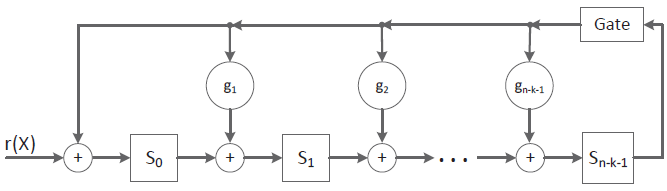
\includegraphics[width=0.8\textwidth]{figures/syndromeCircuit.png}
    \caption{Syndrome calculating circuit}
    \label{fig:syndromeCirc}
\end{figure}



\subsection{Decoder overview}

uml stuff



\fxnote{FIXME: Husk key difficulties her}



\end{document} 